%        File: DesignDocument.tex
%     Created: 一 3月 26 01:00 下午 2018 C
% Last Change: 一 3月 26 01:00 下午 2018 C
%
\documentclass[UTF8,noindent]{ctexart}
\usepackage[a4paper,left=2.0cm,right=2.0cm,top=2.0cm,bottom=2.0cm]{geometry}
\usepackage{hyperref}
\usepackage{url}
\usepackage{graphicx}
\usepackage{amsmath}
\usepackage{amssymb}
\usepackage{enumitem}
\usepackage{tikz}
\usepackage{float}
\usepackage{xeCJK}
\usepackage{listings}
\usepackage{xcolor}
\lstset{language = c,numbers=left, showstringspaces=false,keywordstyle= \color{ blue!70 },commentstyle=\color{red!50!green!50!blue!50}, frame=shadowbox, rulesepcolor= \color{ red!20!green!20!blue!20 } 
} 
\CTEXsetup[format={\Large\bfseries}]{section}
\usetikzlibrary{graphs}
%\newtheorem*{lemma}{Lemma}
\title{\CJKfamily{zhkai}计算机网络研讨课实验报告}
\author{{\CJKfamily{zhkai}冯吕}\ $2015K8009929049$}
\date{\today}
\begin{document}
\maketitle
\zihao{5}
\CJKfamily{zhsong}
%\begin{center}
%  \begin{tabular}{|p{15cm}|}
%    \hline
\section*{{\CJKfamily{zhhei}实验题目}}网络路由实验一。
%\hline
\section*{{\CJKfamily{zhhei}实验内容}}
本次实验需要实现路由器生成和处理$mOSPF\ Hello/LSU$消息的相关操作,
构建一致性链路状态数据库。
\section*{{\CJKfamily{zhhei}实验流程}}
在实验中,需要实现路由器生成和处理$mOSPF\ Hello/LSU$消息的相关操作,构建一致性链路状态数据库,需要实现如下$5$个函数:
\subsection{$sending\_mospf\_hello\_thread$函数}
该函数实现节点广播自己,周期性广播($5s$):发送$mOSPF\ Hello$消息,包括节点$ID$, 端口的子网掩码
目的IP地址为$224.0.0.5$,目的$MAC$地址为$01:00:5E:00:00:05$。
\begin{lstlisting}
void *sending_mospf_hello_thread(void *param)
{
	fprintf(stdout, "TODO: send mOSPF Hello message periodically.\n");
	while (1){
		sleep(MOSPF_DEFAULT_HELLOINT);
		pthread_mutex_lock(&mospf_lock);
		iface_info_t *iface;
		list_for_each_entry(iface, &instance->iface_list, list){
			int len = ETHER_HDR_SIZE + IP_BASE_HDR_SIZE +
			MOSPF_HDR_SIZE + MOSPF_HELLO_SIZE;
			char *hello_packet = (char *)malloc(len);
			struct ether_header *eth = (struct ether_header *)
			hello_packet;
			memcpy(eth->ether_shost, iface->mac, ETH_ALEN);
			u8 dhost[ETH_ALEN] = {0x01, 0x00, 0x5e, 0x00, 0x00, 
			0x05};
			memcpy(eth->ether_dhost, dhost, ETH_ALEN);
			eth->ether_type = htons(ETH_P_IP);

			struct iphdr *iph = packet_to_ip_hdr(hello_packet);
			ip_init_hdr(iph, iface->ip, 0xe0000005, len - 
			ETHER_HDR_SIZE, 90);

			struct mospf_hdr *mohdr = (struct mospf_hdr *)
			(hello_packet + ETHER_HDR_SIZE + IP_BASE_HDR_SIZE);
			mospf_init_hdr(mohdr, 0x1, MOSPF_HDR_SIZE +
			MOSPF_HELLO_SIZE, instance->router_id, 0);

			struct mospf_hello *hello = (struct mospf_hello *)
(hello_packet + ETHER_HDR_SIZE + IP_BASE_HDR_SIZE + MOSPF_HDR_SIZE);
			mospf_init_hello(hello, iface->mask);
			mohdr->checksum = mospf_checksum(mohdr);
			iface_send_packet(iface, hello_packet, len);
		}
		pthread_mutex_unlock(&mospf_lock);
	}
	return NULL;
}
\end{lstlisting}

\subsection{$checking\_nbr\_thread$函数}
该函数实现邻居列表的老化操作,如果列表中的节点在$3*hello-interval$时间内未更新,则将其删除。
\begin{lstlisting}
void *checking_nbr_thread(void *param)
{
	fprintf(stdout, "TODO: neighbor list timeout operation.\n");
	while (1){
		sleep(1);
		pthread_mutex_lock(&mospf_lock);
		iface_info_t *iface;
		list_for_each_entry(iface, &instance->iface_list, list){
			mospf_nbr_t *mos_pos, *mos_q;
			list_for_each_entry_safe(mos_pos, mos_q, 
			&iface->nbr_list, list){
				if (mos_pos->alive > 3 *
				MOSPF_DEFAULT_HELLOINT){
					list_delete_entry(&mos_pos->list);
					free(mos_pos);
					--iface->num_nbr;
				}
				else {
					++mos_pos->alive;
				}
			}
		}
		pthread_mutex_unlock(&mospf_lock);
	}
	return NULL;
}
\end{lstlisting}

\subsection{$handle\_mospf\_hello$函数}
该函数处理$mOSPF\ Hello$消息:
\begin{itemize}
  \item 如果发送该消息的节点不在邻居列表中,添加至邻居列表;
  \item 如果已存在,更新其达到时间;
\end{itemize}
\begin{lstlisting}
void handle_mospf_hello(iface_info_t *iface, const char *packet, int len)
{
	fprintf(stdout, "TODO: handle mOSPF Hello message.\n");
	pthread_mutex_lock(&mospf_lock);
	struct iphdr *iph = packet_to_ip_hdr(packet);
	struct mospf_hdr *moph = (struct mospf_hdr *)(packet + 
	IP_BASE_HDR_SIZE + ETHER_HDR_SIZE);
	struct mospf_hello *hello = (struct mospf_hello *)(packet + 
	ETHER_HDR_SIZE + IP_BASE_HDR_SIZE + MOSPF_HDR_SIZE);

	u32 hello_ip = ntohl(iph->saddr);
	u32 hello_rid = ntohl(moph->rid);
	u32 hello_mask = ntohl(hello->mask);
	mospf_nbr_t *mos_nbr;
	int flag = 0;
	list_for_each_entry(mos_nbr, &iface->nbr_list, list){
		if (mos_nbr->nbr_ip == hello_ip){
			flag = 1;
			mos_nbr->alive = 0;
		}
	}
	if (!flag){
		mospf_nbr_t *new_nbr = (mospf_nbr_t *)
		malloc(sizeof(mospf_nbr_t));
		new_nbr->nbr_id = hello_rid;
		new_nbr->nbr_ip = hello_ip;
		new_nbr->nbr_mask = hello_mask;
		new_nbr->alive = 0;
		list_add_tail(&new_nbr->list, &iface->nbr_list);
		++iface->num_nbr;
	}
	pthread_mutex_unlock(&mospf_lock);
}
\end{lstlisting}

\subsection{$sending\_mospf\_lsu\_thread$函数}
该函数实现节点向每个邻居节点发送链路状态信息,信息包含的内容有:
\begin{itemize}
  \item 该节点$ID (mOSPF\ Header)$、邻居节点$ID$、网络和掩码 ($mOSPF\ LSU$)
	\item 序列号($sequence\ number$),每次生成链路状态信息时加$1$;
	  \item 目的IP地址为邻居节点相应端口的$IP$地址,目的$MAC$地址为邻居节点相应端口
的$MAC$地址;
\end{itemize}
\begin{lstlisting}
void *sending_mospf_lsu_thread(void *param)
{
	fprintf(stdout, "TODO: send mOSPF LSU message periodically.\n");
    while(1){
    	sleep(MOSPF_DEFAULT_LSUINT);

    	pthread_mutex_lock(&mospf_lock);
    	int num_adv = 0;
    	iface_info_t *iface;
    	list_for_each_entry(iface, &(instance->iface_list), list){
    		if(iface->num_nbr == 0)
    			num_adv ++;
    		else
    	        num_adv += iface->num_nbr;
    	}
        int pac_len = ETHER_HDR_SIZE + IP_BASE_HDR_SIZE + MOSPF_HDR_SIZE 
		+ MOSPF_LSU_SIZE + num_adv * MOSPF_LSA_SIZE;
        char *packet = (char *)malloc(pac_len);
        mospf_nbr_t *mos_nbr;
        struct mospf_lsa *mos_lsa;
        int i = 0;
        list_for_each_entry(iface, &(instance->iface_list), list){
        	if(iface->num_nbr == 0){
        		mos_lsa = (struct mospf_lsa *)(packet + pac_len 
				- (num_adv - i) * MOSPF_LSA_SIZE);
        		++i;
        		mos_lsa->subnet = htonl(iface->ip & iface->mask);
        		mos_lsa->mask = htonl(iface->mask);
        		mos_lsa->rid = 0;
        		continue;
        	}
            list_for_each_entry(mos_nbr, &(iface->nbr_list), list){
                mos_lsa = (struct mospf_lsa *)(packet + pac_len 
				- (num_adv - i) * MOSPF_LSA_SIZE);
                ++i;
                mos_lsa->subnet = ntohl(mos_nbr->nbr_ip & mos_nbr->nbr_mask);
                mos_lsa->mask = ntohl(mos_nbr->nbr_mask);
                mos_lsa->rid = ntohl(mos_nbr->nbr_id);
            }
        }
        list_for_each_entry(iface, &(instance->iface_list), list){
            list_for_each_entry(mos_nbr, &(iface->nbr_list), list){
            	char *packet_t = (char *)malloc(pac_len);
            	memcpy(packet_t, packet, pac_len);
            	struct ether_header *eth = (struct ether_header *)packet_t;
                eth->ether_type = htons(ETH_P_IP);       
                memcpy(eth->ether_shost, iface->mac, ETH_ALEN);     

                struct iphdr *iph = (struct iphdr *)(packet_t 
				+ ETHER_HDR_SIZE);
                ip_init_hdr(iph, iface->ip, mos_nbr->nbr_ip, pac_len 
				- ETHER_HDR_SIZE, 90);

                struct mospf_hdr * mospf = (struct mospf_hdr *)(packet_t 
				+ IP_BASE_HDR_SIZE + ETHER_HDR_SIZE);
                mospf_init_hdr(mospf, MOSPF_TYPE_LSU, pac_len 
				- ETHER_HDR_SIZE - IP_BASE_HDR_SIZE, instance->router_id,
			  instance->area_id);  
                
 
                struct mospf_lsu *mos_lsu = (struct mospf_lsu *)
				((char *)mospf + MOSPF_HDR_SIZE);
                mospf_init_lsu(mos_lsu, num_adv);
                mospf->checksum = mospf_checksum(mospf);
                ip_send_packet(packet_t, pac_len);
            }
        	
        }
        instance->sequence_num ++;
        free(packet);
    	pthread_mutex_unlock(&mospf_lock);
    }
	return NULL;
}
\end{lstlisting}

\subsection{$handle\_mospf\_lsu$函数}
该函数处理$mOSF\ LSU$消息:
\begin{itemize}
  \item 如果之前未收到该节点的链路状态信息,或者该信息的序列号更大,则
更新链路状态数据库;
\item $TTL$减1,如果$TTL$值大于$0$,则向除该端口以外的端口转发该消息
\end{itemize}
\begin{lstlisting}
void handle_mospf_lsu(iface_info_t *iface, char *packet, int len)
{
	fprintf(stdout, "TODO: handle mOSPF LSU message.\n");
    mospf_db_entry_t *mos_db_en;
    int flag = 0;
    struct mospf_hdr * mospf = (struct mospf_hdr *)(packet 
	+ IP_BASE_HDR_SIZE + ETHER_HDR_SIZE);
    struct mospf_lsu *mos_lsu = (struct mospf_lsu *)((char *)mospf 
	+ MOSPF_HDR_SIZE);
    struct mospf_lsa *mos_lsa = (struct mospf_lsa *)((char *)mos_lsu 
	+ MOSPF_LSU_SIZE);
    int mospf_rid = ntohl(mospf->rid);
    fprintf(stdout, IP_FMT"\t\n",
				    HOST_IP_FMT_STR(mospf_rid)
			        );
    if(instance->router_id == mospf_rid) return;
    int seq_num = ntohs(mos_lsu->seq);
    int nadv = ntohl(mos_lsu->nadv);
    list_for_each_entry(mos_db_en, &(mospf_db), list){
        if(mospf_rid == mos_db_en->rid && mos_db_en->seq >= seq_num)
        	flag = 1;
        else if(mospf_rid == mos_db_en->rid && mos_db_en->seq < seq_num){
        	flag = 1;
        	free(mos_db_en->array);
        	mos_db_en->array = (struct mospf_lsa *)malloc(nadv 
			* MOSPF_LSA_SIZE);
        	for(int i = 0; i < nadv; i++){
    		    struct mospf_lsa *lsa = (struct mospf_lsa *)(
				(char *)mos_lsa + i * MOSPF_LSA_SIZE);
    		    mos_db_en->array[i].rid = ntohl(lsa->rid);
    		    mos_db_en->array[i].subnet = ntohl(lsa->subnet);
    		    mos_db_en->array[i].mask = ntohl(lsa->mask);
    	    }
        }
    }
    if(! flag){
    	mospf_db_entry_t * mospf_db_en_t = (mospf_db_entry_t *)
		malloc(sizeof(mospf_db_entry_t));
    	mospf_db_en_t->rid = mospf_rid;
    	mospf_db_en_t->seq = seq_num;
    	mospf_db_en_t->nadv = nadv;
    
    	mospf_db_en_t->array = (struct mospf_lsa *)malloc(nadv 
		* MOSPF_LSA_SIZE);
    	for(int i = 0; i < nadv; i++){
    		struct mospf_lsa *lsa = (struct mospf_lsa *)((char 
			*)mos_lsa + i * MOSPF_LSA_SIZE);
    		mospf_db_en_t->array[i].rid = ntohl(lsa->rid);
    		mospf_db_en_t->array[i].subnet = ntohl(lsa->subnet);
    		mospf_db_en_t->array[i].mask = ntohl(lsa->mask);
    	}
    	list_add_tail(&(mospf_db_en_t->list), &mospf_db);
    }
    mospf_db_entry_t *mosdb;
    list_for_each_entry(mosdb, &mospf_db, list){
    	for(int i = 0;i < mosdb->nadv; i++)
    		fprintf(stdout, IP_FMT"\t"IP_FMT"\t"IP_FMT"\t"IP_FMT"\n",
    			    HOST_IP_FMT_STR(mosdb->rid),
				    HOST_IP_FMT_STR(mosdb->array[i].subnet), 
				    HOST_IP_FMT_STR(mosdb->array[i].mask),
				    HOST_IP_FMT_STR(mosdb->array[i].rid)
			        );
    }
    
    mos_lsu->ttl -= 1;
    if(mos_lsu->ttl > 0){
    	iface_info_t *iface_t;
    	mospf_nbr_t *mos_nbr;
    	list_for_each_entry(iface_t, &(instance->iface_list), list){
    		if(iface_t->index == iface->index)
    			continue;
            list_for_each_entry(mos_nbr, &(iface_t->nbr_list), list){
            	char *packet_t = (char *)malloc(len);
            	memcpy(packet_t, packet, len);
            	struct ether_header *eth = (struct ether_header *)packet_t;    
                memcpy(eth->ether_shost, iface_t->mac, ETH_ALEN);
                struct iphdr *iph = (struct iphdr *)(packet_t 
				+ ETHER_HDR_SIZE);
                struct mospf_hdr * mospf = (struct mospf_hdr *)(packet_t 
				+ IP_BASE_HDR_SIZE + ETHER_HDR_SIZE);
                mospf->checksum = mospf_checksum(mospf);
                ip_init_hdr(iph, iface_t->ip, mos_nbr->nbr_ip, len 
				- ETHER_HDR_SIZE, 90);
                ip_send_packet(packet_t, len);
            }
    	}
    }
}
\end{lstlisting}

\subsection{运行实验}
之后,运行实验,在各个路由器节点上运行$mospfd$,使各个节点生成一致的链路状态数据库。
\section*{{\CJKfamily{zhhei}实验结果}}
各个路由器节点生成了一致的链路状态数据库:
\begin{figure}[H]
  \centering
  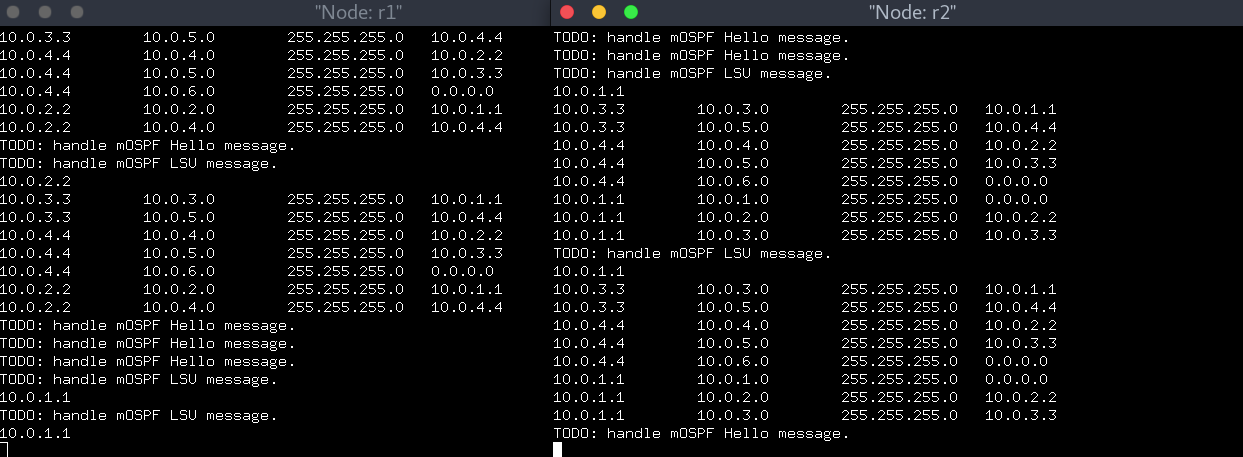
\includegraphics[scale = 0.3]{1.png}
  \caption{运行截图}
\end{figure}

\section*{{\CJKfamily{zhhei}结果分析}}
通过洪泛机制,各个路由器能够生成一致的链路状态数据库,实验结果正确。
\end{document}


